% Springer CCIS / LNCS format -- SPELLL 2026 double-blind submission.
% Derived from ccis_template.tex (LLNCS macro package, v2.21 of 2022/01/12).
\documentclass[runningheads]{llncs}
%
\usepackage[T1]{fontenc}
% T1 fonts will be used to generate the final print and online PDFs,
% so please use T1 fonts in your manuscript whenever possible.
%
\usepackage{amsmath,amssymb,amsfonts}
\usepackage{graphicx}
\usepackage{textcomp}
\usepackage{color}
\usepackage{booktabs}
\usepackage{multirow}
\usepackage{array}
\usepackage{hyperref}
\renewcommand\UrlFont{\color{blue}\rmfamily}
\urlstyle{rm}
\hypersetup{
  hidelinks,
  pdfauthor={},
  pdfsubject={},
  pdfkeywords={}
}

% Custom column type for tables
\newcolumntype{L}[1]{>{\raggedright\arraybackslash}p{#1}}

% Single-column LNCS measure is narrower than the IEEE two-column one; allow
% the line breaker extra slack rather than leaving overfull boxes.
\emergencystretch=2em

% The split-panel figures are taller than LaTeX's default \topfraction (0.7)
% allows, which strands them past the bibliography. Loosen the float rules.
\renewcommand{\topfraction}{0.9}
\renewcommand{\bottomfraction}{0.8}
\renewcommand{\textfraction}{0.07}
\renewcommand{\floatpagefraction}{0.75}

\begin{document}
%
\title{Robust Speaker-Independent Vocal Pathology Detection through Integrated Acoustic and Nonlinear Dynamics}
%
\titlerunning{Robust Speaker-Independent Vocal Pathology Detection}
%
% Double-blind submission: author names, affiliations and e-mail addresses are
% withheld in accordance with the SPELLL 2026 review policy.
\author{Anonymous Author(s)}
%
\authorrunning{Anonymous Author(s)}
%
\institute{Affiliation withheld for double-blind review}
%
\maketitle              % typeset the header of the contribution
%
\begin{abstract}
Voice pathology classification is difficult because pathological speech is nonlinear and varies across time scales, and traditional acoustic metrics describe only part of that behaviour. This paper presents a method for both binary (healthy/pathological) and multi-class (neurological/structural disease group) classification of vocal pathology. It combines multifractal features extracted with Multifractal Detrended Fluctuation Analysis (MFDFA) and standardised acoustic features from the extended Geneva Minimalistic Acoustic Parameter Set (eGeMAPS). Experiments on the Saarbrücken Voice Database use strict speaker-independent cross-validation to rule out speaker-level leakage, a control that much of the earlier literature omits. The method reaches a macro F1 of 0.882 and a balanced accuracy of 0.875 on binary pathology classification, and a macro F1 of 0.637 on disease-group classification, both under five-fold speaker-independent cross-validation. In a feature ablation, the MFDFA features on their own reach an F1 of 0.866.

\keywords{Voice Pathology Detection \and Multifractal Analysis \and Fractal
Dimension \and MF-DFA \and Saarbr\"ucken Voice Database \and Nonlinear Speech
Analysis.}
\end{abstract}
%
%
%
  %--------------------------------------------------------------
  \section{Introduction}
  \label{sec:introduction}
  %--------------------------------------------------------------

Voice disorders are common. They arise from structural pathology of the vocal folds, from neurogenic disorders of motor coordination, and from functional or psychogenic causes. Diagnosis normally combines instrumental procedures such as laryngoscopy with perceptual evaluation by a clinician. That combination is accurate, but perceptual judgement is subjective and demands considerable clinical expertise.

Automatic detection is attractive precisely because it removes that subjectivity. Most systems for recognising pathological voices rely on standard spectral parameters such as MFCCs and F0. These describe the spectral properties of speech well, but they capture little of the temporal and nonlinear behaviour typical of pathological voices.

Speech production is a nonlinear process in which airstream initiation, vocal fold vibration, and articulation all interact. In pathological voices these dynamics can become unstable. Fractal and multifractal theory offers a way to quantify that instability.

This work applies multifractal detrended fluctuation analysis to speech recordings from speakers with diagnosed disorders. Multifractal analysis describes a time series through its scaling properties across time scales. A monofractal signal is characterised by a single scaling exponent; a multifractal one needs a spectrum of local exponents, obtained by varying the moment order $q$ of the analysis.

The question addressed here is whether the multifractal descriptors obtained through MFDFA help detect voice pathology, either on their own or alongside standard acoustic parameters.

  This work differs from earlier fractal-based voice pathology studies in three ways. First, we use the full multifractal spectrum from MFDFA rather than a single scalar fractal dimension, which gives scaling information across several moment orders. Second, one pipeline handles both binary (healthy vs.\ pathological) and multi-class (neurological vs.\ structural) classification, where most earlier studies treat only binary detection. Third, cross-validation is strictly speaker-independent (\texttt{StratifiedGroupKFold}), so recordings from one speaker never appear in both the training and the test split. This guards against the data leakage known to produce optimistic results in much of the earlier literature \cite{saenzlechon2006}. A feature ablation study then quantifies what MFDFA contributes alone and in combination for each classification task.

  %--------------------------------------------------------------
  \section{Related Work}
  \label{sec:related_work}
  %--------------------------------------------------------------

  Automatic detection of voice pathologies has traditionally relied on acoustic features such as MFCCs, perturbation measures, and spectral statistics combined with statistical or machine learning classifiers \cite{godino2006,alnasheri2017,rai2025}. Standardised clinical frameworks have further formalised multi-parameter acoustic assessment: the Dysphonia Severity Index (DSI) combines jitter, phonation time, and intensity into a perceptually anchored score \cite{wuyts2000}, while standardised assessment protocols specify perturbation and noise measures as a clinical evaluation battery \cite{dejonckere2001}. Although these spectral and perturbation-based descriptors capture important phonatory characteristics, they are inherently linear and cannot represent the nonlinear or multi-scale temporal irregularities often present in pathological voices.

  Nonlinear analysis methods have therefore also been explored for pathological speech. Little et al.\ demonstrated that recurrence quantification analysis and fractal scaling properties extracted from sustained phonations can complement conventional acoustic measures for voice disorder detection, achieving correct classification performance above 91\% \cite{little2007b}. Nonlinear dynamical measures such as correlation dimension, Lyapunov exponents, and entropy statistics have been applied to separate healthy from pathological voices with high accuracy on clinical voice databases \cite{henriquez2009,little2007}. Temporal complexity measures therefore carry information that standard spectral descriptors miss. Recurrence plot-based characterisation has also been applied to specific vocal fold pathologies including hyperfunctional dysphonia, laryngitis, and vocal fold polyp, achieving classification accuracy above 90\% on the Saarbrücken Voice Database \cite{krishnan2026}.

  Beyond binary detection, recent work has addressed multi-class voice disorder classification. Orozco-Arroyave et al.\ found that different feature families are required to capture the distinct acoustic signatures of neurological, functional, and laryngeal disorders \cite{orozco2015}. Fractal dimension in multiresolution frameworks has also achieved detection rates above 90\% via per-subband power-spectrum analysis \cite{ali2016,kumar2014}.

  Multifractal detrended fluctuation analysis (MFDFA) extends scalar fractal characterisation by modelling scaling behaviour across multiple moments and time scales \cite{mfdfa}. Multifractal methods have proven effective in other biomedical domains, most notably in demonstrating the multifractal structure of healthy versus diseased heartbeat dynamics \cite{ivanov1999}. Closer to the present work, multifractal analysis has been applied directly to speech signals for glottal activity detection, which shows that the method can capture nonlinear phonatory dynamics \cite{lal2020multifractal}. Speech-based disease detection has also benefited from careful acoustic feature design: Tsanas et al.\ developed 132 dysphonia measures from sustained vowels for high-accuracy Parkinson's disease classification, and showed that engineered descriptors can match or exceed purely data-driven methods in clinical tasks \cite{tsanas2012}. Sai Jahnavi et al.\ likewise detected Parkinson's disease from speech alone using excitation source, voice quality, and prosodic features from sustained vowels \cite{jahnavi2020}. MFDFA applied to voice pathology detection, and particularly to multi-class classification, remains comparatively underexplored.

  One methodological concern cuts across all of this work: speaker-level data leakage. Sáenz-Lechón et al.\ found that systems evaluated without controlling for speaker identity yield optimistic estimates that fail to generalise to unseen speakers, and recommended speaker-independent cross-validation as standard practice \cite{saenzlechon2006}.


  %--------------------------------------------------------------
  \section{Dataset}
  \label{sec:dataset}
  %--------------------------------------------------------------

  The experiments in this study use recordings from the Saarbrücken Voice Database (SVD)~\cite{svd}, a widely used clinical corpus of healthy and pathological voices. The original audio is stored in the proprietary \texttt{.nsp} format and is converted to standard \texttt{.wav} for preprocessing and feature extraction. SVD contains several vowels and connected-speech recordings, but this work uses only the sustained vowel \textit{/a/} at normal pitch (\texttt{a\_n}), which gives a stable phonation condition for cross-speaker comparison.

  Table~\ref{tab:dataset_stats} summarises the dataset used in the experiments.

  \begin{table}[htbp]
  \centering
  \caption{Dataset Statistics}
  \label{tab:dataset_stats}
  \begin{tabular}{ll}
  \toprule
  \textbf{Statistic} & \textbf{Value} \\
  \midrule
  Total recordings (all tokens) & 23,119 \\
  Unique speakers & 1,355 \\
  Pathology classes & 12 (+ healthy) \\
  Samples for token (\texttt{a\_n}) & 1,656 \\
  Sex distribution & 65\% female, 35\% male \\
  \bottomrule
  \end{tabular}
  \end{table}

  The \texttt{a\_n} subset is class-imbalanced, as clinical speech datasets usually are. Pathology classes with too few speakers for reliable speaker-independent cross-validation are excluded. The nine disorders retained span neurological, structural, and functional aetiologies: Parkinson's disease (hypokinetic dysarthria from impaired laryngeal motor control); recurrent laryngeal nerve paralysis (breathiness from vocal fold immobility); spasmodic dysphonia (involuntary voice breaks from laryngeal dystonia); vocal fold nodules (hoarseness from bilateral overuse lesions); vocal fold polyp (breathiness from asymmetric fold vibration); laryngitis (hoarseness from laryngeal mucosal inflammation); hyperfunctional dysphonia (strained voice from excessive laryngeal tension); psychogenic dysphonia (voice disorder of psychological aetiology without organic pathology); and functional dysphonia (dysphonia from maladaptive laryngeal behaviour without an identifiable organic cause).

  \begin{figure}[htbp]
  \centering
  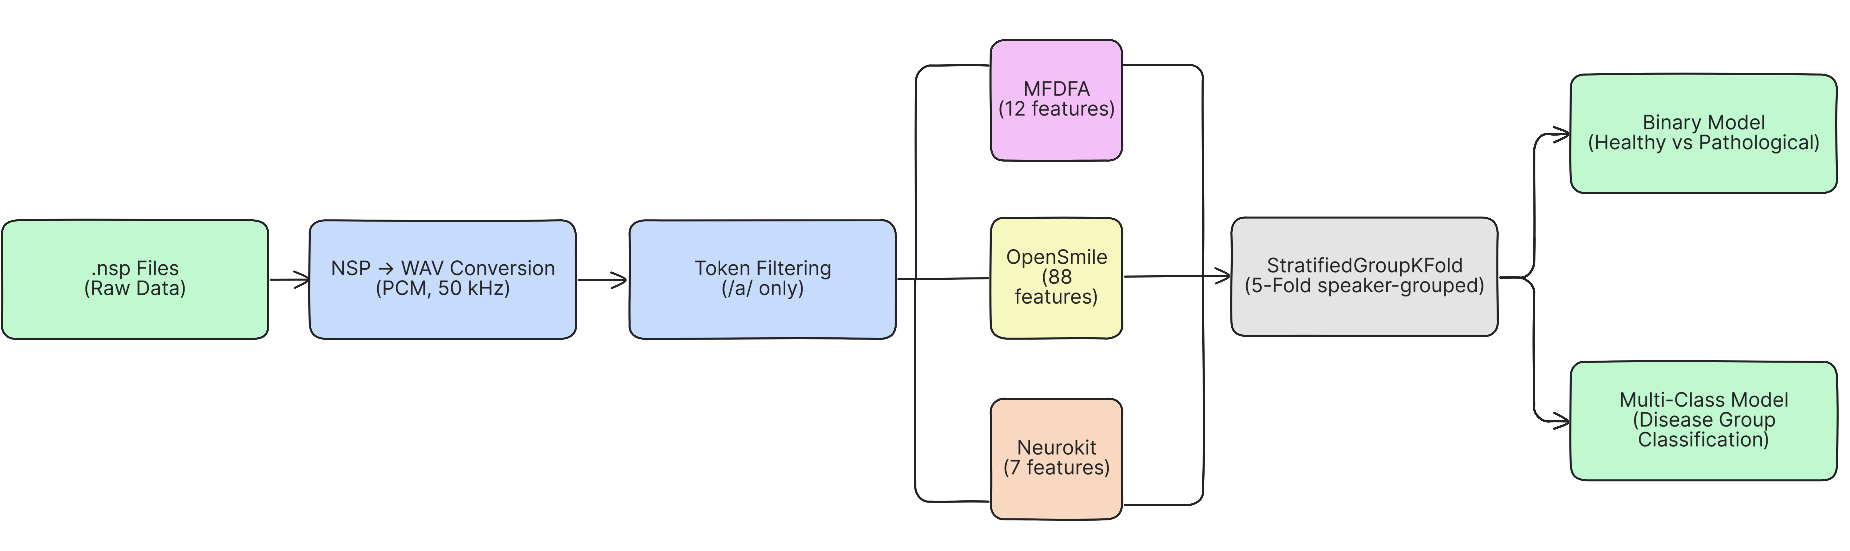
\includegraphics[width=\textwidth]{figures/data_pipeline.png}
  \caption{Overview of the preprocessing and feature extraction pipeline. Raw NSP recordings are converted to WAV format, metadata manifests are generated, and sustained vowel tokens are selected. Multiple feature families are then extracted and merged before training classification models using speaker-grouped cross-validation.}
  \label{fig:data_pipeline}
  \end{figure}

  %--------------------------------------------------------------
  \section{Feature Extraction}
  \label{sec:features}
  %--------------------------------------------------------------

  Four complementary feature families totalling 107 features are extracted from each audio sample: multifractal characteristics, standardised paralinguistic features, nonlinear complexity measures, and speaker metadata.

  \subsection{Multifractal Features}

  Multifractal descriptors capture the nonlinear and multiscale dynamics of pathological speech signals and are extracted with Multifractal Detrended Fluctuation Analysis (MFDFA). Twelve statistical descriptors are derived from the multifractal spectrum, covering the generalised Hurst exponent, the scaling exponent, and the singularity spectrum. The final MFDFA configuration uses first-order detrending, a $q$ range of $[-5,5]$ with step 0.5, and 40 analysis scales.

  \subsection{OpenSMILE Features}

  Standardised acoustic features are extracted with the OpenSMILE toolkit~\cite{opensmile} using the extended Geneva Minimalistic Acoustic Parameter Set (eGeMAPSv02), which contributes 88 parameters covering prosodic, spectral-shape, voice-quality, and temporal characteristics.

  \subsection{NeuroKit2 Features}

  Seven further features are extracted with the NeuroKit2 library to characterise nonlinear signal dynamics, including entropy, fractal-dimension, skewness, and kurtosis measures.

  \subsection{Speaker Metadata}

  Two auxiliary features come from the SVD speaker metadata: age (derived from the recording and birth dates) and biological sex. Both are retained by default across all configurations, and their contribution is examined in the ablation study (Section~\ref{sec:experiments}).

  %--------------------------------------------------------------
  \section{Data Pipeline and Splitting Strategy}
  \label{sec:pipeline}
  %--------------------------------------------------------------

  The overall preprocessing workflow is illustrated in Figure~\ref{fig:data_pipeline}.
  The raw \texttt{.nsp} recordings are converted to \texttt{.wav}, indexed through a metadata manifest, normalised, and then processed by the four feature-extraction modules before the resulting feature tables are merged into a unified machine learning dataset. To minimise variability and within-speaker duplication, most experiments use only the sustained vowel \texttt{a\_n}.

  Speaker-level leakage is the main risk in clinical voice datasets. We therefore use \texttt{StratifiedGroupKFold} with speaker identity as the grouping variable, so all recordings from a speaker stay in the same fold. Rare classes are removed where necessary for stable training, and class imbalance is handled by filtering or downsampling the dominant groups. Final performance is reported as the average over five speaker-grouped folds.
  %--------------------------------------------------------------
  \section{Experimental Setup and Results}
  \label{sec:experiments}
  %--------------------------------------------------------------

  This section evaluates how well the multifractal features discriminate on their own and what they add to conventional acoustic descriptors. All experiments use five-fold speaker-independent cross-validation (\texttt{StratifiedGroupKFold}), so no speaker appears in both the training and the test split. Performance is reported as accuracy, balanced accuracy, and macro-averaged F1; the latter two carry more weight here because of the class imbalance. In preliminary experiments, naive random splits produced far higher scores, which is why every result below uses speaker-independent splits.

  %--------------------------------------------------------------
  \subsection{Speaker-Independent Evaluation}
  %--------------------------------------------------------------

  Only the sustained vowel token \texttt{a\_n} is used to ensure consistency across speakers. Two classification tasks are considered: (1)~binary classification of healthy vs.\ pathological speakers, and (2)~disease-group classification of neurological vs.\ structural disorders.

  The binary task is a screening scenario: decide whether a voice disorder is present. Table~\ref{tab:binary_results} summarises the results under five-fold speaker-grouped cross-validation.

  \begin{table}[htbp]
  \centering
  \caption{Binary Classification Results (Speaker-Grouped CV)}
  \label{tab:binary_results}
  \begin{tabular}{lccc}
  \toprule
  \textbf{Model} & \textbf{Accuracy} & \textbf{Balanced Acc.} & \textbf{F1 Macro} \\
  \midrule
  LightGBM & \textbf{0.889} & 0.875 & \textbf{0.882} \\
  XGBoost & 0.886 & 0.868 & 0.878 \\
  Random Forest & 0.885 & 0.865 & 0.875 \\
  Logistic Regression & 0.875 & 0.867 & 0.870 \\
  \bottomrule
  \end{tabular}
  \end{table}

  These numbers sit well below those from the random-split runs, which is the expected cost of a more realistic protocol. The gradient boosting models, LightGBM and XGBoost, come out ahead, which suggests that nonlinear interactions between features matter for separating pathological from healthy speech.

  Figure~\ref{fig:binary_confmat_models} shows the confusion matrices aggregated across folds. Recall on pathological voices is high, and precision on the healthy class holds up.

  \begin{figure}[htbp]
  \centering
  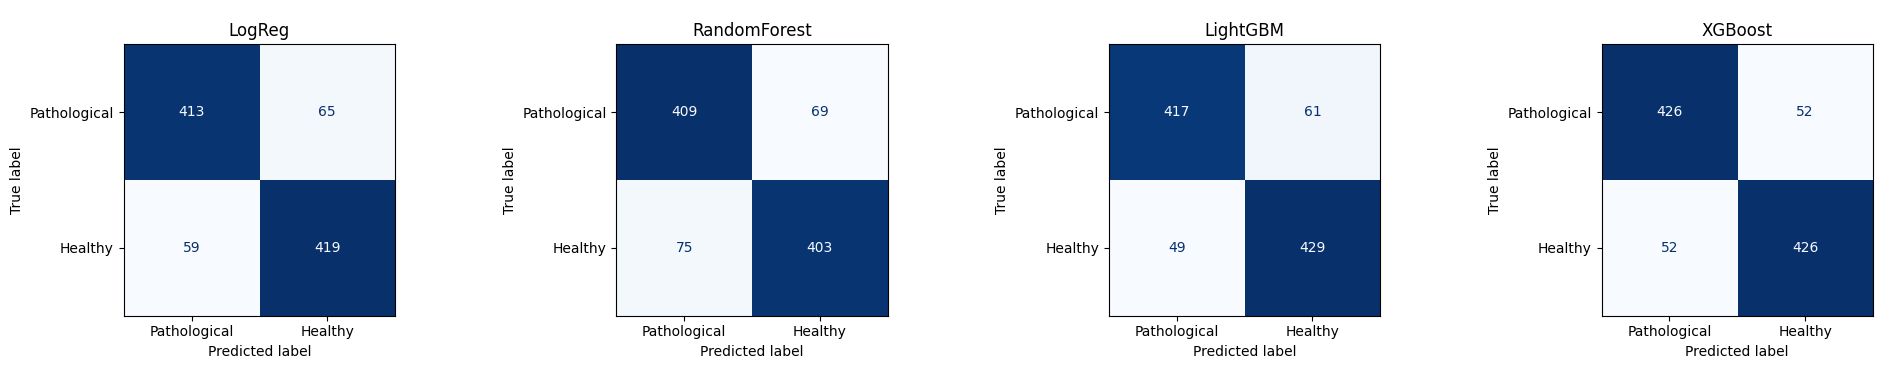
\includegraphics[width=0.49\textwidth,trim={6.48 0 1069.2 0},clip]{figures/binary_confusion_models.png}
  \hfill
  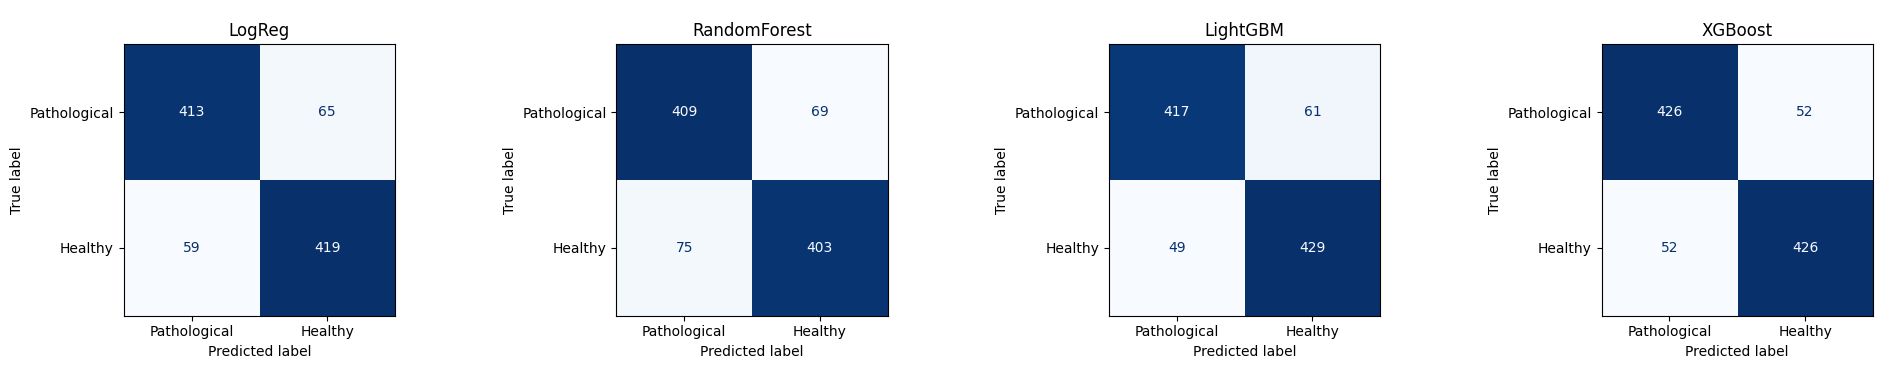
\includegraphics[width=0.49\textwidth,trim={361.44 0 714.24 0},clip]{figures/binary_confusion_models.png}\\[1.5ex]
  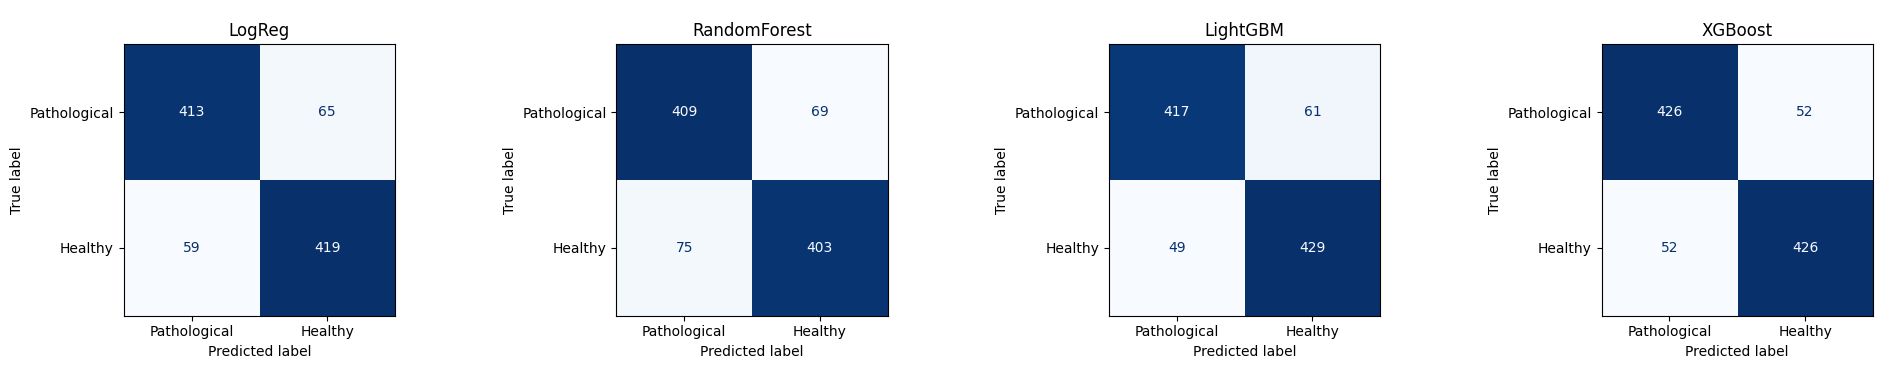
\includegraphics[width=0.49\textwidth,trim={715.68 0 360 0},clip]{figures/binary_confusion_models.png}
  \hfill
  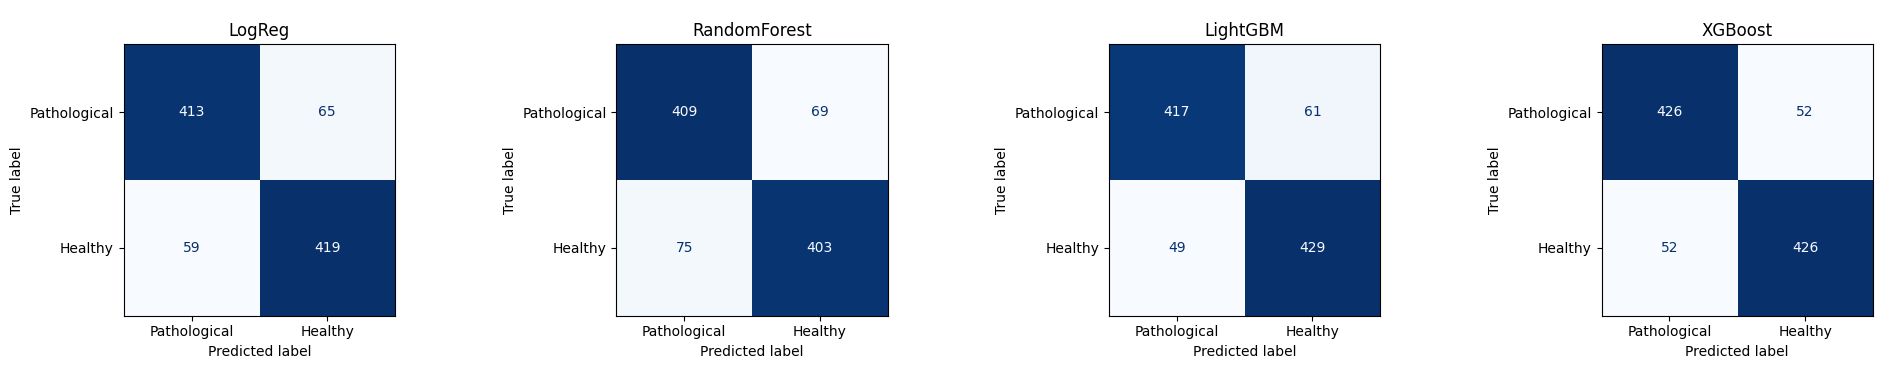
\includegraphics[width=0.49\textwidth,trim={1070.64 0 5.04 0},clip]{figures/binary_confusion_models.png}
  \caption{Cross-validation aggregated confusion matrices for binary classification across different models.}
  \label{fig:binary_confmat_models}
  \end{figure}


  %--------------------------------------------------------------
  \subsection{Disease Group Classification}
  %--------------------------------------------------------------

Detecting pathology is one task. Sorting disorders by clinical cause is a harder one. The pathologies here are split into two clinical categories: neurological and structural.

Neurological disorders come from abnormal neural control of the vocal folds, structural disorders from abnormalities in the tissue of the folds themselves. Separating the two groups from the speech signal alone is difficult.

  Table~\ref{tab:multiclass_results} summarises the performance of the evaluated models for disease-group classification.

  \begin{table}[htbp]
  \centering
  \caption{Disease Group Classification Results}
  \label{tab:multiclass_results}
  \begin{tabular}{lccc}
  \toprule
  \textbf{Model} & \textbf{Accuracy} & \textbf{Balanced Acc.} & \textbf{F1 Macro} \\
  \midrule
  Random Forest & \textbf{0.646} & \textbf{0.628} & \textbf{0.629} \\
  LightGBM & 0.642 & 0.639 & 0.637 \\
  XGBoost & 0.611 & 0.604 & 0.603 \\
  \bottomrule
  \end{tabular}
  \end{table}

  Disease-group classification is much harder than binary pathology detection. The best model reaches an F1 of about 0.63, so the acoustic differences between neurological and structural disorders are far less clear-cut than those between healthy and pathological voices.

  Figure~\ref{fig:multiclass_confusion} illustrates the confusion matrices for this task.

  \begin{figure}[htbp]
  \centering
  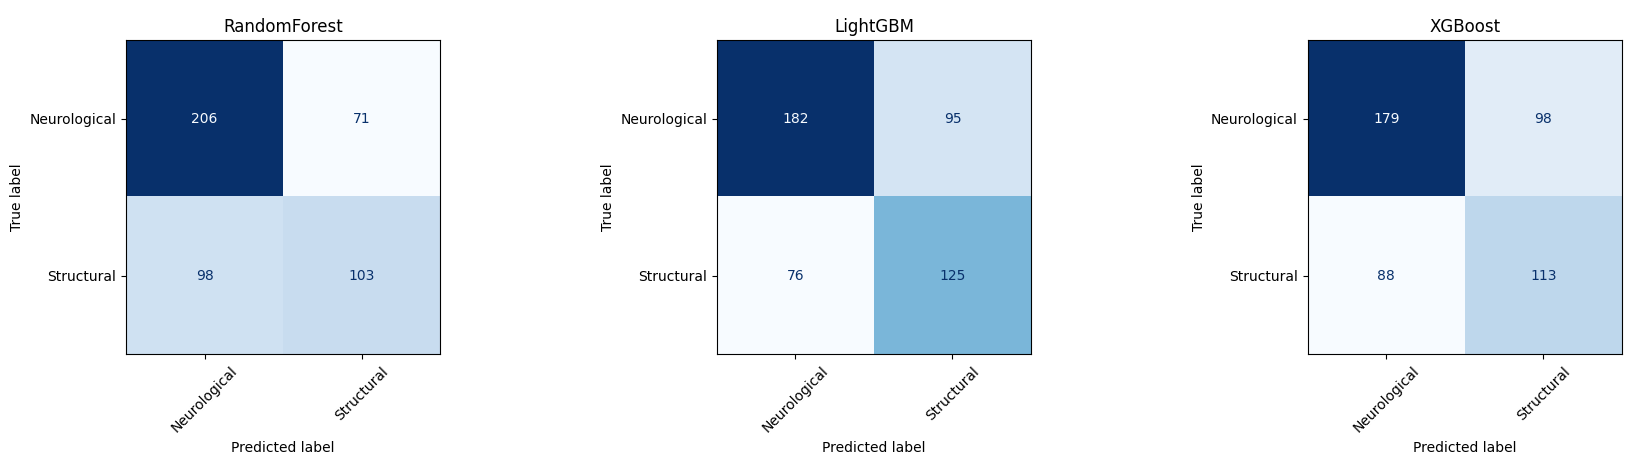
\includegraphics[width=0.49\textwidth,trim={6.75 0 891.75 0},clip]{figures/multiclass_confusion.png}
  \hfill
  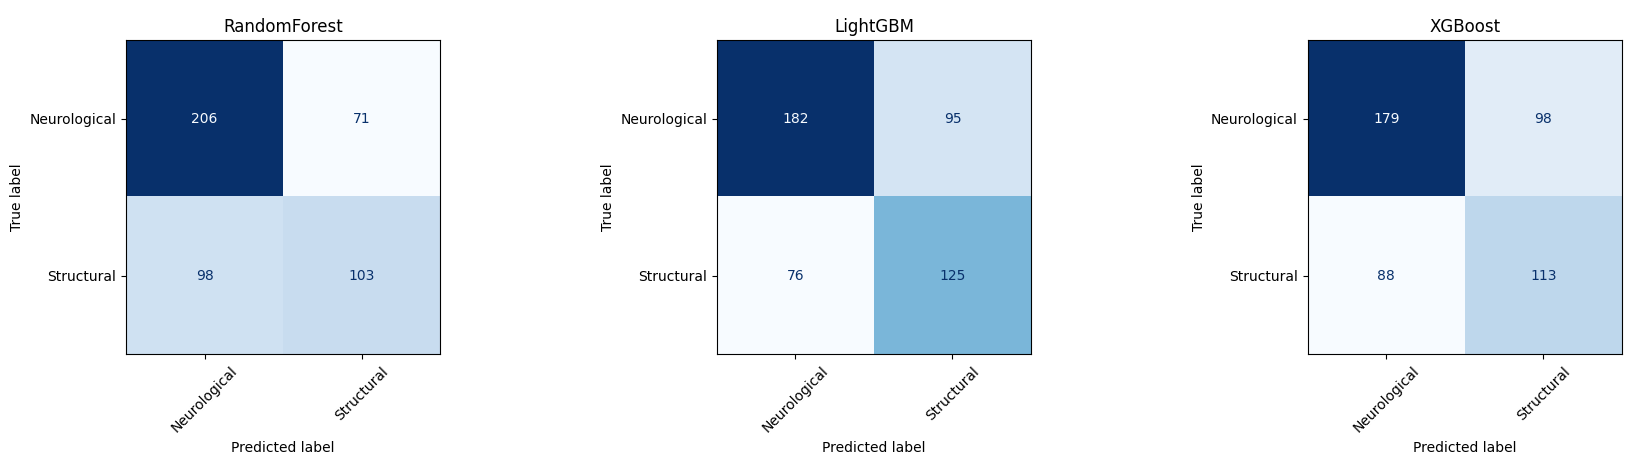
\includegraphics[width=0.49\textwidth,trim={450 0 448.5 0},clip]{figures/multiclass_confusion.png}\\[1.5ex]
  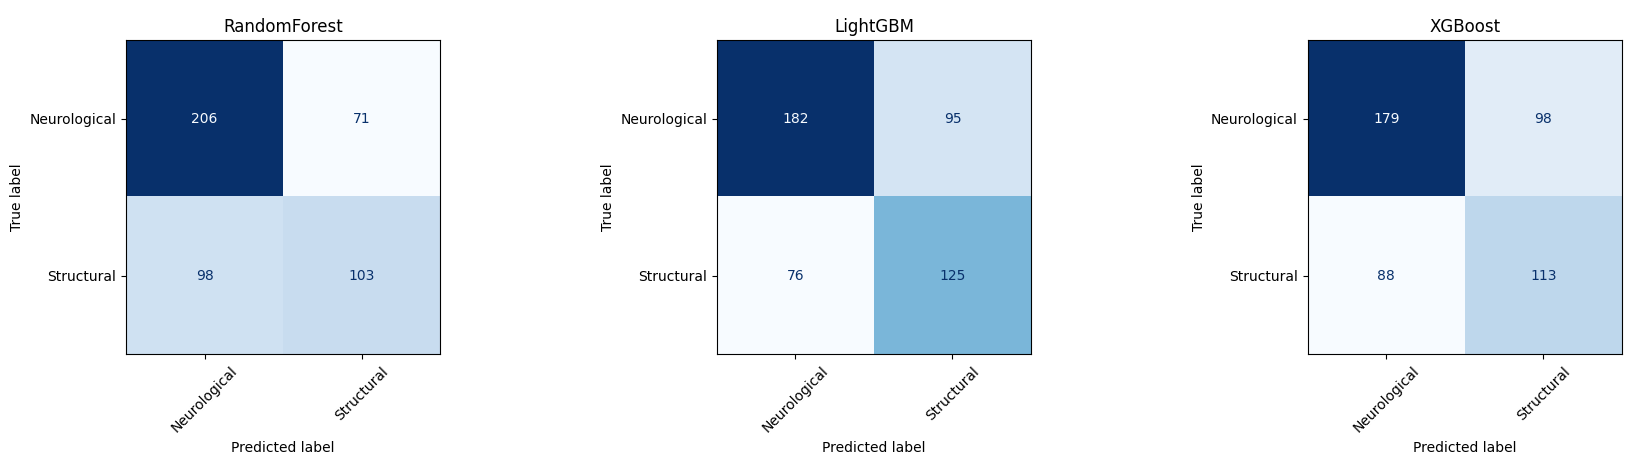
\includegraphics[width=0.49\textwidth,trim={893.25 0 5.25 0},clip]{figures/multiclass_confusion.png}
  \caption{Cross-validation aggregated confusion matrices for multi-class classification across different models.}
  \label{fig:multiclass_confusion}
  \end{figure}

  %--------------------------------------------------------------
  \subsection{Feature Ablation Analysis}
  %--------------------------------------------------------------

  A feature ablation study measures what each feature family contributes. Combinations of multifractal features, OpenSMILE descriptors, and NeuroKit2 features were evaluated under the same speaker-grouped cross-validation protocol. All configurations include the speaker metadata (age and biological sex) unless stated otherwise. The final row of Table~\ref{tab:ablation_binary} isolates the effect of removing age from the best configuration.

  \begin{table}[htbp]
  \centering
  \caption{Feature Ablation Results (Binary Classification)}
  \label{tab:ablation_binary}
  \begin{tabular}{L{5.4cm} L{2.4cm} c c}
  \toprule
  \textbf{Feature Configuration} & \textbf{Best Model} & \textbf{Bal.\ Acc.} & \textbf{F1 Macro} \\
  \midrule
  MFDFA + OpenSMILE & LightGBM & \textbf{0.879} & \textbf{0.878} \\
  MFDFA + NeuroKit2 + OpenSMILE & XGBoost & 0.876 & 0.876 \\
  MFDFA + NeuroKit2 & LogReg & 0.868 & 0.867 \\
  MFDFA only & LogReg & 0.867 & 0.866 \\
  MFDFA + OpenSMILE $-$ Age & LightGBM & 0.752 & 0.749 \\
  \bottomrule
  \end{tabular}
  \end{table}

  \begin{figure}[htbp]
  \centering
  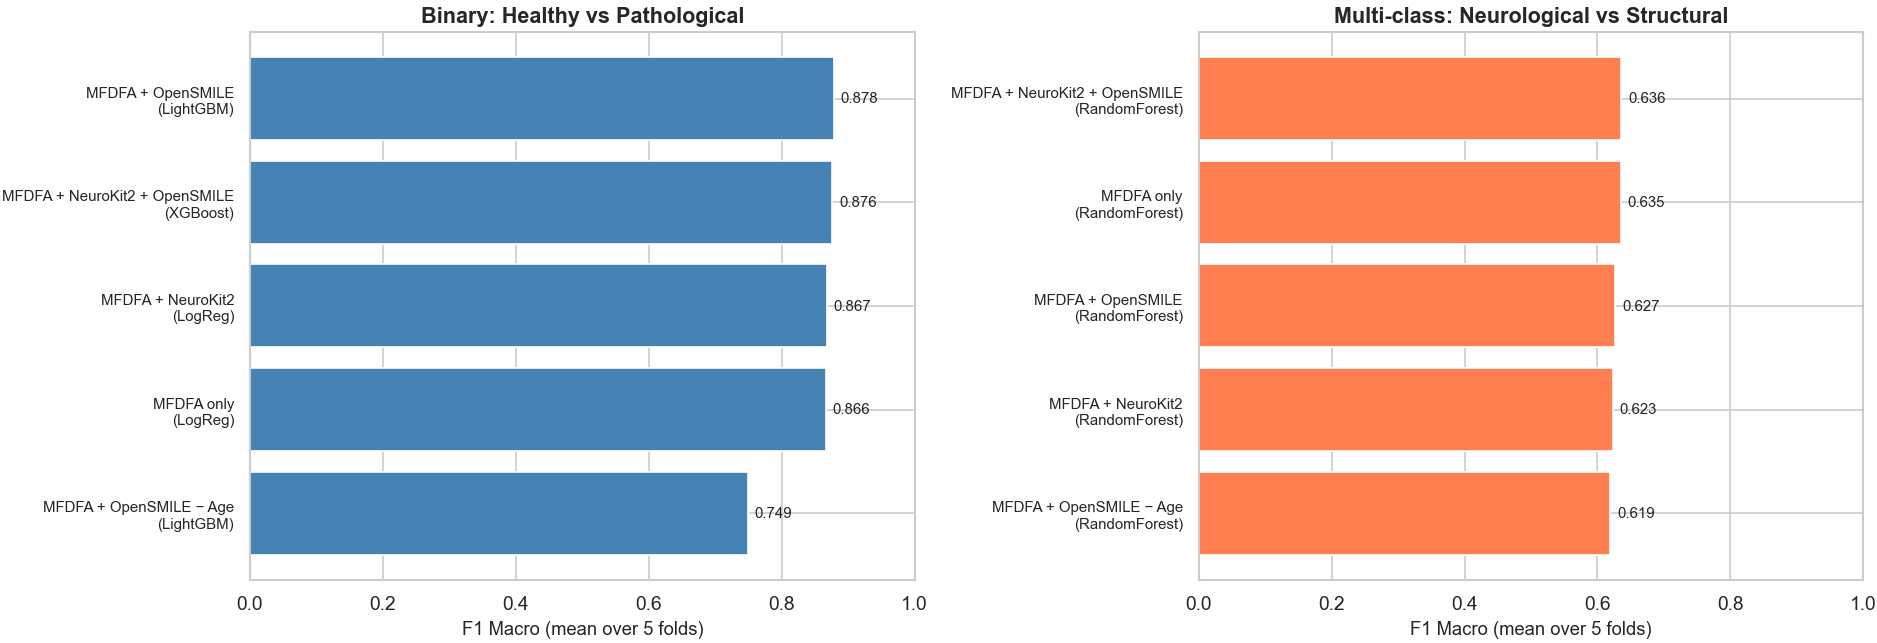
\includegraphics[width=\textwidth,trim={1.8 0 570.6 0},clip]{figures/feature_ablation.png}\\[1.5ex]
  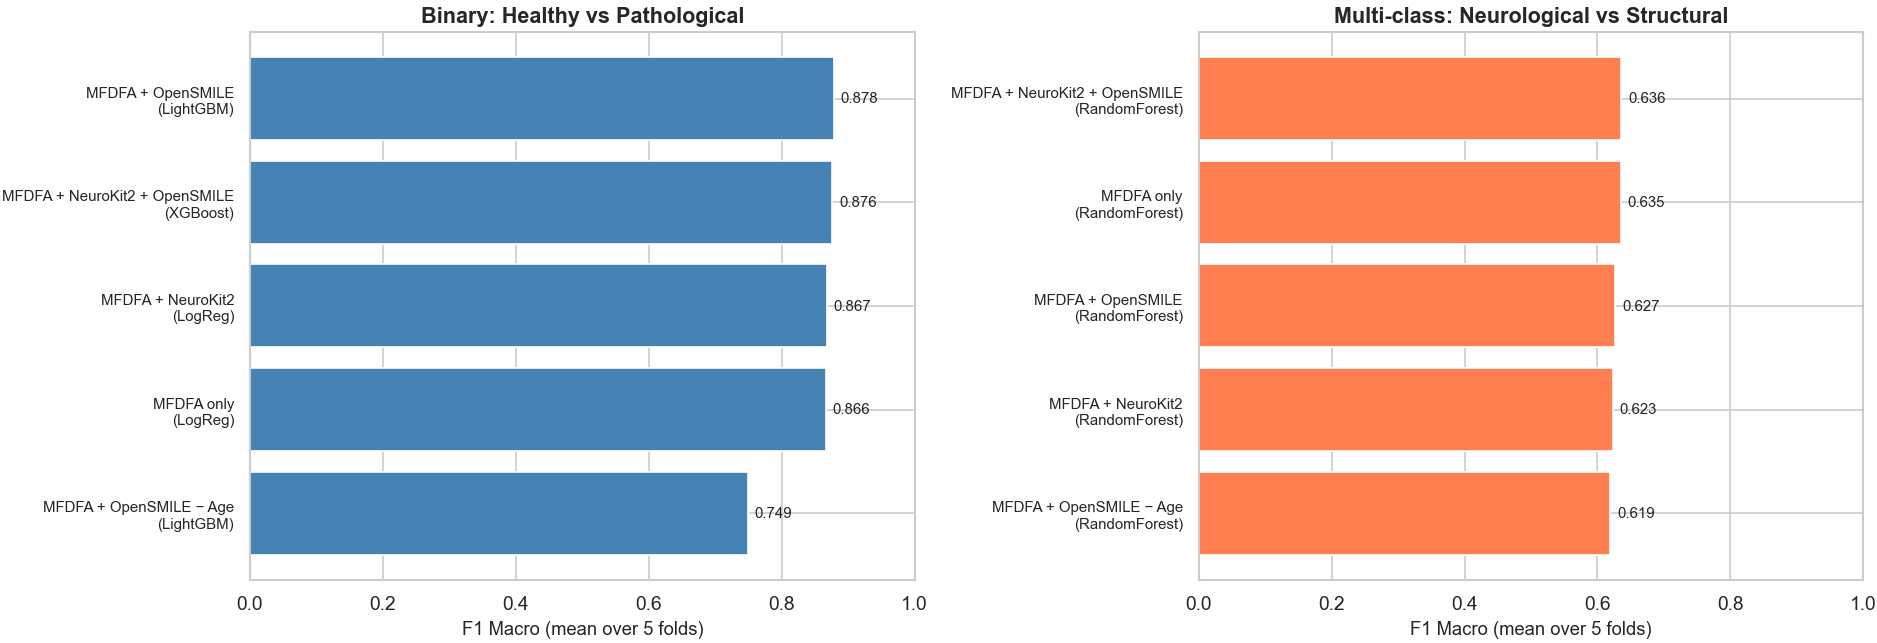
\includegraphics[width=\textwidth,trim={571.2 0 1.2 0},clip]{figures/feature_ablation.png}
  \caption{Feature ablation results for binary and multi-class classification.}
  \label{fig:ablation_results}
  \end{figure}

The multifractal features on their own reach an F1 of 0.866, so much of what separates healthy from pathological phonation is already present in the scaling behaviour of the signal. Adding the OpenSMILE features lifts this to 0.878, a small gain that suggests the two families are partly complementary.

Adding NeuroKit2 changes almost nothing, so the complexity information it measures is largely already captured by the multifractal descriptors.

Age has a much larger effect than any of that. Dropping it from the MFDFA+OpenSMILE model costs 0.129 macro F1, from 0.878 down to 0.749. Age is therefore strongly associated with the labels in this dataset, and any interpretation of the acoustic results has to account for it. Figure~\ref{fig:ablation_results} compares all configurations.

  %--------------------------------------------------------------
  \subsection{Per-Disease Binary Detection}
  %--------------------------------------------------------------

  A separate binary classifier was trained for each disease against the healthy class to see which pathologies are individually detectable.

  \begin{table}[htbp]
  \centering
  \caption{Per-Disease Binary Detection Results}
  \label{tab:per_disease}
  \begin{tabular}{L{5.4cm} L{2.4cm} c c}
  \toprule
  \textbf{Disease} & \textbf{Best Model} & \textbf{Bal.\ Acc.} & \textbf{F1 Macro} \\
  \midrule
  Recurrent Laryngeal Nerve Paralysis & XGBoost & \textbf{0.866} & \textbf{0.865} \\
  Reinke's Edema & LightGBM & 0.829 & 0.828 \\
  Laryngitis & XGBoost & 0.796 & 0.796 \\
  Vocal Fold Polyp & LightGBM & 0.795 & 0.793 \\
  Functional Dysphonia & XGBoost & 0.794 & 0.794 \\
  Psychogenic Dysphonia & XGBoost & 0.790 & 0.788 \\
  Hyperfunctional Dysphonia & XGBoost & 0.773 & 0.773 \\
  Spasmodic Dysphonia & LightGBM & 0.617 & 0.587 \\
  Vocal Fold Nodules & Random Forest & 0.531 & 0.485 \\
  \bottomrule
  \end{tabular}
  \end{table}

  Recurrent laryngeal nerve paralysis and Reinke's edema are the most acoustically distinct. Vocal fold nodules and spasmodic dysphonia are the hardest, at 0.531 and 0.617 balanced accuracy, which we attribute to their subtle acoustic manifestation and to small sample sizes. Screening for pathology in general is reliable; identifying which pathology is not, and closing that gap will likely need larger and more specialised datasets.


  %--------------------------------------------------------------
  \section{Conclusion}
  \label{sec:conclusion}
  %--------------------------------------------------------------

  This paper investigates multifractal descriptors obtained via MFDFA for automated voice pathology detection on the Saarbrücken Voice Database. MFDFA features are combined with conventional acoustic (OpenSMILE) and complexity-based (NeuroKit2) descriptors and evaluated under strict speaker-independent cross-validation, so the reported scores apply to unseen speakers.

  Binary pathology detection reaches a macro F1 of 0.882, and the ablation shows that the MFDFA descriptors alone reach 0.866 without any conventional acoustic features. Disease-group classification is considerably weaker at 0.637 macro F1, and per-disease detection ranges from 0.865 down to 0.485 F1. For now the method suits screening better than differential diagnosis.

  Next steps are validation on larger independent cohorts, extension to multiple tokens and to end-to-end models, and an analysis of which parts of the multifractal spectrum carry the clinically useful signal.

%--------------------------------------------------------------
% References -- Springer 'splncs04' style, generated by BibTeX from refs.bib.
% Build: pdflatex paper_ccis && bibtex paper_ccis && pdflatex paper_ccis (x2)
% splncs04.bst sorts alphabetically by first author, so reference numbers do
% NOT follow order of citation. That is correct for LNCS/CCIS.
% Ship paper_ccis.bbl alongside the source; Springer requires it.
%--------------------------------------------------------------
\bibliographystyle{splncs04}
\bibliography{refs}
\end{document}
